\documentclass{book}
\usepackage{commeunjeustyle}

\begin{document}

\section*{Equation différentielle d'ordre 1}
\begin{Exercice}[Premier ordre, à coefficients constants]
Résoudre les équations différentielles suivantes :
\begin{enumerate}
\item $x'+x=1$
\item $7x'+2x=-5t^2+4t-1$
\item $x'+2x=t^2-2t+3$
\item $x'+x=te^{-t}$
\item $x'-2x=\cos(t)$
\end{enumerate}
\end{Exercice}
\begin{Exercice}[Datation]
Le carbone 14 possède plusieurs isotopes dont le carbone 14 -
noté $C^{14}$, utilisé pour la datation. La proportion de carbone 14 est constante
chez un organisme vivant. Après sa mort, la vitesse de disparition du carbone 14
est proportionnelle à la proportion de $C^{14}$ présente dans l'organisme. On note
$k$ la constante de proportionnalité.
\begin{enumerate}
\item On note $x(t)$ la proportion de $C^{14}$ à un instant t dans l'organisme. Écrire
l'équation différentielle satisfaite par $x$.
\item Résoudre l'équation différentielle.
\item On appelle période de demi-vie la durée nécessaire pour que la proportion
de $C^{14}$ ait diminuée de moitié. Sachant que la période de demi-vie du $C^{14}$
est de 40 ans, calculer la constante k.
\item Une équipe d'archéologues a mesuré dans une momie une proportion de
$C^{14}$ de $9,15.10^{?38}$. A quelle dynastie appartient ce pharaon ()?
\end{enumerate}
\end{Exercice}
%%%%%%%%%%%
\begin{Exercice}[Equation différentielle linéaire de premier ordre]
\label{exo:1}
Résoudre les équations différentielles suivantes :
  
\begin{enumerate}
\item Sur $\R$ : $$E_1 :  \, x'+ x= \cos t+\sin t$$

Puis déterminer la solution au problème de Cauchy : 
$$\begin{cases}
x'+ x= \cos t+\sin t  \\
 x(0) = 2  \\
\end{cases}$$

\item Sur $\R$ : $$ E_2 : \, x'-2t x= \mathrm{sh} t   -   2  t   \mathrm{ch} t$$

\item Sur $\R^*_+$ : $$E_3 : \, tx'+(t-1)x= t^2$$
\end{enumerate}
\begin{Correction}
\begin{enumerate}
\item %Sur $\R, \, E_1 :   x'+ x= \cos t + \sin t$.

	\begin{enumerate}
	\item Résolvons l'équation homogène $(H) : \; x' = - x$ , associée à $(E)$.
		\begin{itemize}

			\item Posons $a(t) = -1$, $a$ est définie et continue sur $\R$.

%On cherche une primitive $A$ de $a$ sur l'intervalle $\R$ :
%\hspace{0.7cm} $a(x) = -\frac{1}{2} \times \frac{2x}{1+x^2}$ on reconnait une forme $\frac{u'}{u}$ avec $u(x)=1+x^2$.
%Donc une primitive est :

				\hspace{0.7cm} $A(t) =  - t$ primitive de $a$ sur $\R$

			\item La solution générale de $(H)$ est  :

				%\hspace{0.7cm} $x_0 = C \mathrm{e}^{ \frac{1}{2} \ln(1+x^2)}$ où $C \in \R$	

				\hspace{0.7cm} $x_0 = C  \mathrm{e}^{-t} $ où $C \in \R$	
		\end{itemize}


	\item Par superposition des solutions, il suffit de trouver une solution particulière à $x'+ x= \cos t $ d'une part et  à $x'+ x= \sin t$ d'autre part, pour déterminer une solution particulière à $(E)$.

	De plus par linéarité, il suffit de trouver une solution particulière à $x' + x = \mathrm{e}^{\mathrm{i} t}$ pour trouver les solutions particulières ci-dessus.


	\item Déterminons une solution particulière à $x' + x = \mathrm{e}^{\mathrm{i} t}$ par la méthode de la variation de la constante.

	Posons $\lambda \in \mathcal{D}(\R ,\R)$ et cherchons une solution sous la forme :

		\hspace{0.7cm} $x_{1} = \lambda(t) \mathrm{e}^{-t}$  \hspace{0.5cm} $x_{1}$ est dérivable comme produit de fonctions dérivables et :

		\hspace{0.7cm} $x'_{1} = \lambda'  \mathrm{e}^{-t} - \lambda   \mathrm{e}^{-t}$

	Donc :

\hspace{0.7cm} $x_{1} \text{ solution } 
\Longleftrightarrow 
x'_{1} + x_{1} = \mathrm{e}^{\mathrm{i} t}$

\hspace{0.7cm} $\phantom{x_{1} \text{ solution } } 
\Longleftrightarrow
 \lambda'  \mathrm{e}^{-t} - \lambda   \mathrm{e}^{-t}  + 
  \lambda   \mathrm{e}^{-t} = \mathrm{e}^{\mathrm{i} t}$
 
\hspace{0.7cm} $\phantom{x_{1} \text{ solution } } 
\Longleftrightarrow
 \lambda'  \mathrm{e}^{-t} =  \mathrm{e}^{\mathrm{i} t}$
 
		  \hspace{0.7cm} $\phantom{x_{1} \text{ solution }  } \Longleftrightarrow
 \lambda' = \mathrm{e}^{ (1+\mathrm{i}) t}$
 
		 Donc : $\lambda = \tfrac{1}{1+\mathrm{i}}  \mathrm{e}^{ (1+\mathrm{i}) t}$ convient et une solution particulière est :

  		\hspace{0.7cm} $x_{1} =  \tfrac{1}{1+\mathrm{i}}  \mathrm{e}^{ \mathrm{i} t}$
  
    	\hspace{0.7cm} $\phantom{ x_{1} } =  \tfrac{1- \mathrm{i}}{2}  \mathrm{e}^{ \mathrm{i} t}$

    	\hspace{0.7cm} $\phantom{ x_{1} } =  \tfrac{\cos t + \sin t}{2} +  \mathrm{i} \tfrac{- \cos t + \sin t}{2}$
    

	\item Solutions particulières à :
		\begin{itemize}
    		\item $x' + x = \cos t$ : $\mathcal{R}e ( x_1 ) =  \tfrac{\cos t + \sin t}{2}$
    
    		\item $x' + x = \sin t$ : $\mathcal{I}m ( x_1 ) =  \tfrac{- \cos t + \sin t}{2}$
    	\end{itemize}    
    
      
	\item Solution générale de $(E)$ :
    
    		\hspace{0.7cm} $x = C \mathrm{e}^{- t}  + \tfrac{\cos t + \sin t}{2} + \tfrac{- \cos t + \sin t}{2}$   où $C \in \R$.

    		\hspace{0.7cm} $x = C \mathrm{e}^{- t}  + \sin t$   où $C \in \R$.
    
	\item Résolution du problème de Cauchx :

    	\hspace{0.7cm} $x(0)=2 \Longleftrightarrow C + 0 = 2$
    
	    \hspace{0.7cm} $\phantom{x(0)=2} \Longleftrightarrow C = 2$   
    
	Donc la solution au problème de Cauchy est  : 

       \hspace{0.7cm} $x = 2\mathrm{e}^{- t}  +  \sin t$
	\end{enumerate}

Vous avez la méthode et une rédaction (trop) détaillée\dots pour la suite je vous donne les résultats.



\item %Sur $\R, \, E_2 :  x'-2t x= \mathrm{sh} t   -   2  t   \mathrm{ch} t$.

	\begin{enumerate}
		\item Solution générale de l'équation homogène associée $(H) : \, x' = 2t x$ :

			\hspace{0.7cm} $x_0 = C  \mathrm{e}^{t^2} $ où $C \in \R$	

		\item Solution particulière  de $(E_2)$ : (il faut le \og voir  \fg{} à la forme de l'équation)

			\hspace{0.7cm} $x_1 = \mathrm{ch} t$ 

		\item Solution générale de $(E)$ :
    
		    \hspace{0.7cm} $x = C \mathrm{e}^{t^2}  +\mathrm{ch} t$   où $C \in \R$.
	\end{enumerate}


\item %Sur $\R^*_+ , \, E_3 tx'+(t-1)x= t^2$.

	\begin{enumerate}
		\item On normalise, c'est possible sur $\R^*_+$ : 
		
			\hspace{0.7cm} $x'+ \frac{t-1}{t} x= t$
	
		\item Solution générale de l'équation homogène associée $(H) : \, x' = - \frac{t-1}{t} x$ :

			\hspace{0.7cm} $x_0 = C t  \mathrm{e}^{-t} $ où $C \in \R$	

		\item Solution particulière  de $(E_3)$ :

			\hspace{0.7cm} $x_1 = t$ 

		\item Solution générale de $(E)$ :
    
		    \hspace{0.7cm} $x = C t  \mathrm{e}^{-t}  + t$   où $C \in \R$.
	\end{enumerate}
\end{enumerate}
\end{Correction}
\end{Exercice}
\begin{Exercice}[\'Equation différentielle linéaire de premier ordre non homogène]
Résoudre les équations différentielles suivantes :
$$tx'(t) + x(t) = 0 (I = \mathbb{R})$$
$$ 2t x'(t) + x(t) = t^2 (I = \mathbb{R})$$
$$ (1+t^2)^2x'(t) + 2tx(t) = t e^{\frac{1}{1+t^2}}$$
\end{Exercice}

\begin{Exercice}[Varions la constante...]
Résoudre les équations différentielles suivantes :
\begin{enumerate}
\item $x'+x=\frac{1}{1+e^t}$ sur $\mathbb R$;
\item $(1+t)x'+x=1+\ln(1+t)$ sur $]-1,+\infty[$;
\item $x'-\frac xt=t^2$ sur $]0,+\infty[$;
\item $x'-2tx=-(2t-1)e^t$ sur $\mathbb R$;
\item $x'-\frac{2}tx=t^2$ sur $]0,+\infty[$;
\end{enumerate}
\end{Exercice}
\begin{Exercice}[Raccordement des solutions- tous les cas possibles]
Déterminer les solutions sur $\mathbb R$ des équations différentielles suivantes :
\begin{enumerate}
\item $tx'-2x=t^3$;
\item $t^2x'-x=0$;
\item $(1-t)x'-x=t$;
\item $(1 + t)x' ? x = t^2+2t+2$
\end{enumerate}
\end{Exercice}
\section*{Systèmes différentiels linéaires }
\begin{Exercice}[Diagonalisable]
Résoudre le système suivant :
$$ x'(t) = 5 x(t) -3y(t)$$
$$ y'(t) = 6 x(t) -4y(t)$$
\end{Exercice}
\begin{Exercice}[Triangulaire supérieur]
Résoudre le système suivant :
$$ x'(t) = x(t)  + y(t)$$
$$ y'(t) =   y(t)$$
\end{Exercice}
\begin{Exercice}[Champs magnétique]
Le mouvement d'une particule chargée dans un champ magnétique suivant l'axe $(Oz)$
est régi par un système différentiel de la forme
$$\left\{
\begin{array}{rcl}
x''&=&\omega y'\\
y''&=&-\omega x'\\
z''&=&0
\end{array}\right.$$
où $\omega$ dépend de la masse et de la charge de la particule, ainsi que du champ magnétique. 
En posant $u=x'+iy'$, résoudre ce système différentiel.
\end{Exercice}
\begin{Exercice}[Diagonalisable]
Donner le système différentiel suivant :
$$\begin{cases}
x' &= x+2y-z \\
y' &= 2x+4y?2z\\
z' &= -x-2y+z
\end{cases}$$
\end{Exercice}
\begin{Exercice}[Un peu de physique: étude du mouvement d'un système de masses reliées par des ressorts, glissant le long d'une poutre soufflante]
Pour simplifier, les ressorts ont même raideur k et les corps même masse m.
Notons $x_i(t)$ l'écart par rapport à la position d'équilibre pour le i-ème corps.\\
\begin{center}
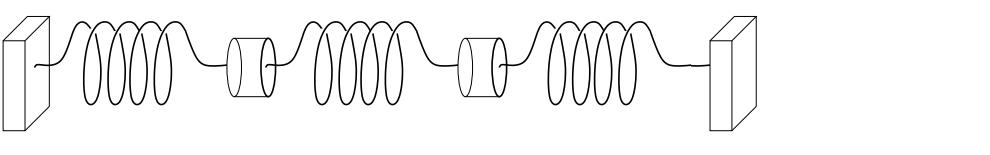
\includegraphics[width=12cm]{resort.png}\\
\end{center}
Le principe fondamentale s'écrit :
$$m x_1''(t) = -2k.x_1(t)  +k.x_2(t)$$
$$m x_2''(t) = k.x_1(t)  - 2k.x_2(t)$$
\begin{enumerate}
\item Modéliser ce système linéaire sous forme matricielle;
\item Résoudre le système ;
\item Les physiciens ont compris qu'en général, le mouvement est une superposition de mouvements
fondamentaux appelés modes propres. Ce sont les mouvements où tous les corps oscillent à la
même fréquence. Déterminer les fréquences propres $w$ du système. 
\end{enumerate}
\end{Exercice}
%
%%%%%%%%%%%
\section*{Équations différentielles linéaires scalaires du second ordre}
\begin{Exercice}[\'Equations du second ordre à coefficients constants]
Résoudre les équations différentielles suivantes :
\begin{enumerate}
\item $x''-2x'+x=t$, $x(0)=x'(0)=0$;
\item $x''+9x=t+1$, $x(0)=0$;
\item $x''-2x'+x=\sin^2 t$;
\end{enumerate}
\end{Exercice}
\begin{Exercice}[Equation différentielle linéaire de second ordre]
Résoudre les équations différentielles suivantes  :   
\begin{enumerate}
\item Sur $\R$ :
$$E_1 : \, x''+2x'-3x = 11   \mathrm{e}^{2t}      $$ % ???? \dfrac{1}{\mathrm{e}^{2t}+1}$ 

\item Sur $[0 ; \pi[$
 $$E_2 : \, x''+x=  \cos t                  $$  %\dfrac{1}{\cos t}$

\item Sur $\R$
$$E_3 : \, x''-2x'+x = \mathrm{ch} t$$

\item Sur $\R$ :
$$E_4 : \, x'' + x'+2x = 6 e^{2t}    $$ 

\item Sur $\R$ :
$$E_5 : \, x'' +  2x'+5x = \cos t    $$

\item Sur $\R$ :
$$E_6 : \, x'' - x = \sh t    $$ 
\end{enumerate} 
\begin{Correction}
Résoudre les équations différentielles suivantes  :   
\begin{enumerate}
\item %Sur $\R, \, E_1 : x''+2x'-3x = 11   \mathrm{e}^{2t}      $ % ???? \dfrac{1}{\mathrm{e}^{2t}+1}$ 
	\begin{enumerate}
		\item  \'Equation différentielle homogène associée :  \, $ (H) \,x'' + 2x' - 3x = 0 $

			polynôme caractéristique associé : $x^2  + 2x - 3 = 0$.
			
			Discriminant : $\Delta = 16 > 0$

			Racines du polynôme : $x_1 = 1$ et $x_2 =  - 3$.

			La solution générale de $(H)$ est : 
			
			\hspace{0.7cm} $x_H = A \mathrm{e}^{t} + B  \mathrm{e}^{-3t}$, avec $A,B \in \R$.

		\item Détermination une solution particulière à $(E)$, comme $2$ n'est pas racine du polynôme caractéristique on la cherche sous la forme $x_1 = C \mathrm{e}^{2t}$ où $C \in \R$, qui est deux fois dérivables sur $\R$ :
		
			\hspace{0.7cm} $x'_1 = 2C \mathrm{e}^{2t}$

			\hspace{0.7cm} $x''_1 = 4C \mathrm{e}^{2t}$
			
		\hspace{0.7cm} $x_{1} \text{ solution de } (E) \Longleftrightarrow x''_{1} +2 x'_1 - 3x_{1} = 11\mathrm{e}^{2x}$

		\hspace{0.7cm} $\phantom{x_{1} \text{ solution de } (E)} \Longleftrightarrow  \dots$
		
		\hspace{0.7cm} $\phantom{x_{1} \text{ solution de } (E)} \Longleftrightarrow C=\tfrac{11}{5}$
		
		\hspace{0.7cm} $x_{1} = \tfrac{11}{5} \mathrm{e}^{2t} $ solution de $(E)$.
		
		\item Solution générale de $(E)$ :
		
		\hspace{0.7cm} $x = A \mathrm{e}^{t} + B  \mathrm{e}^{-3t} + \tfrac{11}{5} \mathrm{e}^{2t} $, avec $A,B \in \R$.	
	\end{enumerate}

\item % Sur $[0 ; \pi[, \, E_2 : x''+x=  \cos t                   $  %\dfrac{1}{\cos t}$
	\begin{enumerate}
		\item  \'Equation différentielle homogène associée :  \, $ (H) \,x'' + x = 0 $

			\dots

			La solution générale de $(H)$ est : 
			
			\hspace{0.7cm} $x_H = A \cos t + B  \sin t $, avec $A,B \in \R$.

		\item On détermine une solution particulière à $(\tilde{E}) x''+x=  \mathrm{e}^{\mathrm{i}t}$ et une solution particulière de $(E)$ sera, par linéarité, la partie réelle de la solution trouvée.
		
Attention, comme $\mathrm{i}$ est racine simple du polynôme caractéristique on la cherche sous la forme $x_1 = C t \mathrm{e}^{\mathrm{i}  t}$ avec $C \in \R$, qui est deux fois dérivables sur $\R$ :
		
		\dots
		
		\hspace{0.7cm} $x_{1} = \tfrac{\mathrm{i}}{2} t \mathrm{e}^{\mathrm{i} t} $ solution de $(\tilde{E})$.

		\dots
		
		\hspace{0.7cm} $x_{2} = -\tfrac{ t }{2} \sin t $ solution de $( E )$.		
		
		\item Solution générale de $(E)$ :
		
		\hspace{0.7cm} $x =  A \cos t + B  \sin t - \tfrac{ t }{2} \sin t $, avec $A,B \in \R$.	
	\end{enumerate}

\item %Sur $\R, \, E_3 : x''-2x'+x = \mathrm{ch} t$
	\begin{enumerate}
		\item  \'Equation différentielle homogène associée :  \, $ (H) \,x'' -2x' + x = 0 $

			\dots

			La solution générale de $(H)$ est : 
			
			\hspace{0.7cm} $x_H = A  \mathrm{e}^{t} + B t  \mathrm{e}^{-t}$, avec $A,B \in \R$.

		\item On détermine une solution particulière $x_1$ à $(E_1)  x''-2x'+x =  \mathrm{e}^{ t }$, puis $x_2$ à $(E_2)  x''-2x'+x =  \mathrm{e}^{ -t }$ et une solution particulière de $(E)$ sera, par superposition, $\frac{x_1 + x_2}{2}$.
		
Attention, comme $1$ est racine double du polynôme caractéristique on cherche $x_1$ sous la forme $x_1 = C t^2 \mathrm{e}^{ t}$ avec $C \in \R$, qui est deux fois dérivables sur $\R$ :
		
		\dots
		
		\hspace{0.7cm} $x_{1} = \tfrac{ 1 }{2} t^2 \mathrm{e}^{ t} $ solution de $(E_1)$.

		\dots
		
		\hspace{0.7cm} $x_{2} = \tfrac{ 1 }{4}  \mathrm{e}^{ -t} $ solution de $( E_2 )$.		

		\dots
		
		\hspace{0.7cm} $x_{3} = \tfrac{ 1 }{4} t^2 \mathrm{e}^{ t}  + \tfrac{ 1 }{8}  \mathrm{e}^{ -t} $ solution de $( E_2 )$.	
		
		\item Solution générale de $(E)$ :
		
		\hspace{0.7cm} $x =   A  \mathrm{e}^{t} + B t  \mathrm{e}^{-t} +  \tfrac{ 1 }{4} t^2 \mathrm{e}^{ t}  + \tfrac{ 1 }{8}  \mathrm{e}^{ -t}$, avec $A,B \in \R$.	
	\end{enumerate}
\end{enumerate} 
\end{Correction}
\end{Exercice}
\begin{Exercice}[Changement de variable]
On cherche à résoudre sur $\mathbb R_+^*$ l'équation di?érentielle :
$$x^2y''-3xy'+4y = 0.\ (E)$$
\begin{enumerate}
\item Cette équation est-elle linéaire ? Qu'est-ce qui change par rapport au cours ?
\item Analyse. Soit $y$ une solution de $(E)$ sur $\mathbb R_+^*$. Pour $t\in\mathbb R$, on pose $z(t)=y(e^t)$.
\begin{enumerate}
\item Calculer pour $t\in\mathbb R$, $z'(t)$ et $z''(t)$.
\item En déduire que $z$ vérifie une équation différentielle linéaire d'ordre 2 à coefficients  constants que l'on précisera (on pourra poser $x = e^t$ dans $(E)$). 
\item Résoudre l'équation différentielle trouvée à la question précédente.
\item En déduire le "portrait robot" de $y$.
\end{enumerate}
\item Synthèse. Vérifier que, réciproquement, les fonctions trouvées à la ?n de l?analyse sont bien toutes les solutions de (E) et conclure.
\end{enumerate}
\end{Exercice}
\begin{Exercice}[Dissolution]
La vitesse de dissolution d'un composé chimique dans l'eau est proportionnelle à la quantité restante. On place 20g de ce composé, et on observe que 5min plus tard, il reste 10g. Dans combien de temps restera-t-il seulement 1g?
\end{Exercice}
\begin{Exercice}[Séparation des variables]
On considère l'équation différentielle
$$y'-e^t e^y=0$$
Déterminer ses solutions, en précisant soigneusement leurs intervalles de définition.
\end{Exercice}
\begin{Exercice}[Développement en série entière]
Pour les équations différentielles suivantes :
\begin{itemize}
\item Chercher les solutions développables en séries entières
\item Résoudre complètement l'équation sur un intervalle bien choisi par la méthode d'abaissement de l'ordre
\item Résoudre l'équation sur $\mathbb{R}$ :
\end{itemize}
$$ t(t-1)x''+3tx'+x=0.$$
\end{Exercice}

\end{document}
